\documentclass[11pt]{article}

\usepackage[a4paper, margin=1.05in]{geometry}
\usepackage{amsmath, amssymb, amsthm, mathtools}
\usepackage{graphicx}
\usepackage{booktabs}
\usepackage{microtype}
\usepackage{xcolor}
\usepackage{enumitem}
\usepackage{tikz}
\usetikzlibrary{arrows.meta, positioning}
\usepackage[numbers]{natbib}
\usepackage[hypertexnames=false]{hyperref}
\hypersetup{colorlinks=true, linkcolor=black!55!blue,
  citecolor=black!55!blue, urlcolor=black!45!blue}
\sloppy \emergencystretch=2.5em

\newtheorem{lemma}{Lemma}
\newtheorem{claim}{Claim}
\theoremstyle{definition}
\newtheorem{question}{Question}
\newtheorem*{answer}{Answer}
\theoremstyle{remark}
\newtheorem{remark}{Remark}

\newcommand{\R}{\mathbb{R}}
\newcommand{\N}{\mathcal{N}}
\newcommand{\E}{\mathbb{E}}
\newcommand{\dd}{\mathrm{d}}
\newcommand{\T}{^{\!\top}}
\newcommand{\given}{\,|\,}
\DeclareMathOperator{\Var}{Var}
\DeclareMathOperator{\Cov}{Cov}
\DeclareMathOperator{\tr}{tr}

\tikzset{
  var/.style={circle, draw=black!70, fill=white, line width=0.8pt,
              minimum size=7.5mm, inner sep=0pt},
  fac/.style={rectangle, draw=black!70, fill=black!12, line width=0.8pt,
              minimum size=4.5mm, inner sep=2pt},
  obs/.style={rectangle, draw=red!60!black, fill=red!12, line width=0.8pt,
              minimum size=4.5mm, inner sep=2pt},
  e/.style={line width=0.8pt, black!60},
}

\title{\bfseries Belief Propagation for the Gaussian AR(1) Diffusion Model,\\
Equation by Equation\\[4pt]
\large From continuous messages to two-number updates, AMP,\\
and the price of locality}
\author{Giovanni Mantovani\\[2pt]
\small Bocconi University, MSc Data Science\\[1pt]
\small working note following the call with J.~Garnier-Brun, 5 June 2026}
\date{\today}

\begin{document}
\maketitle

\begin{abstract}
\noindent
This note does one thing slowly and completely: it derives belief propagation
(BP) for the Gaussian AR(1) diffusion model \emph{equation by equation},
assuming nothing as known. It is organised around the points raised in the
call of 5~June~2026: (i) BP messages are probability distributions, and for
continuous variables they are \emph{functions} --- numerically intractable to
propagate as such; (ii) the practical resolution is to parametrise each
message as a Gaussian and update two numbers, a mean and a variance --- the
construction known as AMP in computer science and TAP in physics; (iii) the
proposed checkpoint: run BP with Gaussian messages on the model we can solve
exactly, and check it recovers the known score; (iv) the proposed
experiments: truncate the exact score matrix to a band, and separately cut
the message iteration to a local range, and quantify the damage relative to
the full computation; compare the Gaussian local-field approximation (AMP)
against the exact score. We construct the factor graph from zero, write
every sum--product update, compute every integral in display, and prove that
for this model the Gaussian parametrisation is not an approximation: the
update equations map Gaussians to Gaussians \emph{exactly}, so two-number
messages run BP without loss --- the checkpoint passes at $10^{-14}$. We
then answer the call's open questions: the messages are exactly Gaussian
here because every update is a linear-Gaussian operation; node-wise Gaussian
messages do \emph{not} in general imply a Gaussian joint law, but here the
joint posterior is Gaussian for a separate reason (its log-density is a
quadratic form); and the central-limit objection --- ``a CLT on two points is
usually not right'' --- does not bite the BP mean (no averaging is invoked)
but does bite the AMP \emph{variance} closure, whose per-node update loses
its fixed point beyond a measurable diffusion time. Experiments: truncating
the score to tridiagonal costs up to $\sim30\%$ relative RMS error at
intermediate diffusion times and almost nothing at very small or very large
times; cutting the message range to $r$ hops behaves the same way but is
strictly better than matrix banding at small times --- truncated
\emph{inference} renormalises where truncated \emph{matrices} do not. All
numbers are produced by a self-contained, self-checking code
(\texttt{bp\_gaussian.py}) and an executed companion notebook.
\end{abstract}

\tableofcontents
\medskip\hrule\medskip

% =============================================================================
\section{What this note is, and where it comes from}\label{sec:origin}
% =============================================================================

This note is a from-scratch reconstruction. Its agenda is fixed by the call
of 5~June~2026 with J.~Garnier-Brun, and by nothing else. The points made in
that call, in the order they will drive the document:

\begin{enumerate}[leftmargin=1.7em, itemsep=2pt]
\item \textbf{The continuous-message problem.} BP messages are probability
distributions. With discrete variables a message is a finite vector of
probabilities --- easy to store, easy to normalise, easy to update. With
continuous variables a message is ``theoretically a function over the entire
support'': the update rules become integrals, and the normalisation constant
of every message would need to be recomputed at every step. Propagating
functions numerically is the obstruction.
\item \textbf{The resolution to try.} Declare that the distribution being
propagated is Gaussian, ``and since it's Gaussian, then I can describe it
with the mean and the variance \dots\ then what you do is that you update
the mean and the variance.'' This two-number reduction is the step called
\emph{tapification}; the resulting algorithm family is AMP (approximate
message passing) in computer science, the TAP equations in physics.
\item \textbf{The doubt.} The Gaussian form of a message is usually
justified by a central limit theorem: at a factor node that aggregates
\emph{many} incoming messages, their sum is approximately Gaussian. Our
factor graph is the opposite --- ``very tree-like, like a straight line with
things on the side'' --- and every update takes essentially \emph{two}
inputs. ``The central limit theorem on two data points is usually not
right.'' Separately: even if the distribution on each node is Gaussian, it
is ``not entirely trivial'' that the joint distribution of the whole
sequence is Gaussian.
\item \textbf{The checkpoint.} ``Go back to the case where $a_{k+1}$ equals
something times $a_k$ plus a Gaussian. You knew how to solve it, you solved
it. Can we actually do this with a message-passing algorithm? \dots\ the
actual Gaussianity assumption on the BP messages, in the Gaussian data case
\dots\ and see if we recover what we had.''
\item \textbf{The experiments.} (a)~``Imagine you take the exact score and,
instead of using the full matrix, you truncate it to the tridiagonal thing
--- how bad is the approximation?'' (b)~With BP one can do better than
truncating a matrix: ``you restrain your factor graph \dots\ you cut the
iteration at some point \dots\ the nodes are updated in such a way that we
don't actually run through the entire graph, but we do local approximations
every time. And then how bad is the inference compared to the real thing?''
(c)~The Gaussian local-field scheme (AMP) against the exact score.
\item \textbf{Why it matters.} The inference on every node requires
propagating messages through the entire sequence --- ``clearly it's not
local,'' which is the same observation as ``the denoising matrix is not
tridiagonal, it's actually full.'' But if, in some region of diffusion time,
local inference is close to correct, ``you could restrain the architecture
very strongly \dots\ instead of having a fully connected model, [have] one
that does patches, like a CNN.''
\end{enumerate}

\noindent Nothing in what follows is assumed known. Every object is defined
before it is used; every equation is derived where it appears; every claim
that can be checked numerically is checked, by the self-contained code in
this folder.

% =============================================================================
\section{The model, every symbol defined}\label{sec:model}
% =============================================================================

\paragraph{The data.} A \emph{sequence} is a vector of $K$ real numbers
$a=(a_0,a_1,\dots,a_{K-1})\in\R^K$. We call $k$ the \emph{frame index}. The
sequence is random, generated by the first-order autoregressive (AR(1)) rule
\begin{equation}\label{eq:ar1}
  a_{k+1}\;=\;\alpha\,a_k\;+\;\eta_k,
  \qquad \eta_k\sim\N(0,\sigma_\eta^2)\ \text{independent of everything},
  \qquad |\alpha|<1 .
\end{equation}
Here $\alpha$ is a fixed number measuring how strongly one frame remembers
the previous one, and $\eta_k$ is fresh Gaussian noise injected at every
step. We start the chain at $a_0\sim\N(0,\sigma_0^2)$.

\paragraph{Choice of constants.} We choose
\begin{equation}\label{eq:stationary}
  \sigma_0^2=1,
  \qquad
  \sigma_\eta^2=1-\alpha^2 .
\end{equation}
This is the \emph{stationary, unit-variance} normalisation, and it is a
choice, not a necessity. Why it is convenient: if $\Var(a_k)=1$, then by
\eqref{eq:ar1} and independence of $\eta_k$,
\[
  \Var(a_{k+1})=\alpha^2\Var(a_k)+\sigma_\eta^2
  =\alpha^2+(1-\alpha^2)=1 ,
\]
so every frame has variance exactly $1$: the chain looks statistically the
same at every position, and no formula below needs to carry $k$-dependent
variances.

\paragraph{The corruption (diffusion channel).} Diffusion models destroy
data with noise and learn to reverse the destruction. At \emph{diffusion
time} $t\ge0$ (a second time axis, completely distinct from the frame index
$k$), each frame is independently corrupted:
\begin{equation}\label{eq:channel}
  x_k\;=\;e^{-t}\,a_k\;+\;\xi_k,
  \qquad \xi_k\sim\N(0,D_t)\ \text{i.i.d.},
  \qquad D_t:=1-e^{-2t}.
\end{equation}
The number $e^{-t}$ shrinks the signal; $D_t$ is the variance of the added
noise. The pair is matched so that
$\Var(x_k)=e^{-2t}\cdot1+D_t=1$ at every $t$: the channel is
\emph{variance-preserving}. At $t=0$, $x_k=a_k$ (nothing happened); as
$t\to\infty$, $x_k$ becomes pure $\N(0,1)$ noise (everything happened).

\paragraph{The object to compute.} Write $P_t(x)$ for the probability
density of the noisy sequence $x=(x_0,\dots,x_{K-1})$. The \emph{joint
score} is its log-gradient,
\begin{equation}\label{eq:score-def}
  S(x,t)\;:=\;\nabla_x\log P_t(x)\;\in\;\R^K .
\end{equation}
This is the function a diffusion model must learn: it is the drift that the
reverse-time (generative) process adds to undo the noise, and the
Bayes-optimal denoiser is an affine function of it (made exact in
Step~\ref{step:tweedie} below). ``Joint'' matters: $S_k$ is the derivative
of the log-density of the \emph{whole} sequence with respect to $x_k$, and
it will turn out to depend on every frame, not just on $x_k$.

% =============================================================================
\section{The exact answer, derived from zero}\label{sec:exact}
% =============================================================================

Before any algorithm, we need the ground truth that the algorithms will be
judged against. Everything in this section is elementary probability,
written out in full.

\paragraph{Step 3.1: the clean covariance.}\label{step:cov}
Iterating \eqref{eq:ar1} from frame $j$ up to frame $i>j$,
\[
  a_i=\alpha^{\,i-j}a_j+\underbrace{\textstyle\sum_{l=j}^{i-1}
  \alpha^{\,i-1-l}\,\eta_l}_{\text{independent of }a_j} .
\]
Multiplying by $a_j$ and taking expectations (the noise terms are
independent of $a_j$ and have mean zero),
\[
  \E[a_ia_j]=\alpha^{\,i-j}\,\E[a_j^2]=\alpha^{\,i-j}\cdot 1 .
\]
By symmetry, for any $i,j$:
\begin{equation}\label{eq:Sigma0}
  (\Sigma_0)_{ij}:=\Cov(a_i,a_j)=\alpha^{|i-j|} .
\end{equation}
The clean law is the centred Gaussian $P_0(a)=\N(a;0,\Sigma_0)$ --- Gaussian
because $a$ is a linear function of the i.i.d.\ Gaussian variables
$(a_0,\eta_0,\eta_1,\dots)$.

\paragraph{Step 3.2: the noisy covariance and the exact score.}
Stack \eqref{eq:channel} as $x=e^{-t}a+\xi$ with $\xi\sim\N(0,D_tI)$
independent of $a$. Then $x$ is again Gaussian and centred, with
\begin{equation}\label{eq:Sigmat}
  \Sigma_t:=\Cov(x)=e^{-2t}\,\Sigma_0+D_t\,I .
\end{equation}
The log-density of a centred Gaussian is
$\log P_t(x)=-\tfrac12\,x\T\Sigma_t^{-1}x+\text{const}$, and for a symmetric
matrix $A$ one has $\nabla_x(x\T A x)=2Ax$ (differentiate the double sum
$\sum_{ij}A_{ij}x_ix_j$ with respect to $x_k$: the terms containing $x_k$
are $A_{kk}x_k^2$ and $\sum_{j\ne k}(A_{kj}+A_{jk})x_kx_j$, giving
$2\sum_jA_{kj}x_j$). Hence
\begin{equation}\label{eq:score-exact}
  \boxed{\;S(x,t)=-\,\Sigma_t^{-1}x\;}
\end{equation}
This is the benchmark: one $K\times K$ linear solve. The score is a
\emph{linear} function of $x$, and its coupling pattern is the matrix
$Q_t:=\Sigma_t^{-1}$, which is \emph{dense} for $t>0$ --- this density is
exactly the non-locality that the call's experiments are about.

\paragraph{Step 3.3: the score as a denoiser (Tweedie's identity).}
\label{step:tweedie}
The same score can be computed without ever forming $\Sigma_t$, through the
posterior over the clean sequence. Write the channel density
\[
  p_t(x\given a)=\prod_{k=0}^{K-1}
  \frac{1}{\sqrt{2\pi D_t}}\exp\!\Big(-\frac{(x_k-e^{-t}a_k)^2}{2D_t}\Big),
  \qquad
  P_t(x)=\int_{\R^K}P_0(a)\,p_t(x\given a)\,\dd a .
\]
Differentiate $P_t$ under the integral sign with respect to $x_k$ (allowed:
the integrand is smooth and dominated). Only the $k$-th channel factor
depends on $x_k$, and
\[
  \partial_{x_k}\,p_t(x\given a)
  =-\frac{x_k-e^{-t}a_k}{D_t}\;p_t(x\given a) .
\]
Therefore
\[
  \partial_{x_k}P_t(x)
  =-\frac1{D_t}\int\big(x_k-e^{-t}a_k\big)\,P_0(a)\,p_t(x\given a)\,\dd a .
\]
Now divide by $P_t(x)$ and recognise Bayes' rule:
$P_0(a)\,p_t(x\given a)/P_t(x)=p(a\given x)$, the \emph{posterior} density
of the clean sequence given the noisy one. The ratio of integrals becomes a
posterior expectation:
\begin{equation}\label{eq:tweedie}
  \boxed{\;S_k(x,t)=\partial_{x_k}\log P_t(x)
  =\frac{e^{-t}\,\E[a_k\given x]\;-\;x_k}{D_t}\;}
\end{equation}
Read it: the $k$-th score component is, up to known constants, the gap
between the noisy frame and the channel-attenuated \emph{best estimate of
the clean frame given the whole noisy sequence}. Computing the score
\emph{is} computing the Bayesian denoiser $\E[a_k\given x]$ --- this is the
form a message-passing algorithm will target, because $\E[a_k\given x]$ is
a per-node posterior mean, which is exactly what BP computes.

\paragraph{Step 3.4: the posterior, explicitly.}\label{step:posterior}
We will need $p(a\given x)$ itself. Up to factors that do not depend on
$a$,
\[
  -\log p(a\given x)
  =\tfrac12\,a\T Q_0\,a
  +\sum_{k=0}^{K-1}\frac{(x_k-e^{-t}a_k)^2}{2D_t}
  +\text{const},
  \qquad Q_0:=\Sigma_0^{-1}.
\]
Expanding the channel squares and collecting powers of $a$: each one
contributes $\frac{e^{-2t}}{2D_t}a_k^2$ (quadratic) and
$-\frac{e^{-t}}{D_t}x_ka_k$ (linear). Hence
\begin{equation}\label{eq:posterior}
  p(a\given x)\ \propto\
  \exp\!\Big(-\tfrac12\,a\T J\,a+h\T a\Big),
  \qquad
  J=\frac{e^{-2t}}{D_t}I+Q_0,
  \qquad
  h=\frac{e^{-t}}{D_t}\,x ,
\end{equation}
a Gaussian with mean $m=J^{-1}h$ and covariance $J^{-1}$ (complete the
square: $-\tfrac12a\T Ja+h\T a=-\tfrac12(a-m)\T J(a-m)+\text{const}$).
Substituting $m$ into \eqref{eq:tweedie} and simplifying recovers
\eqref{eq:score-exact} --- the code checks this identity at $10^{-15}$
rather than trusting the algebra.

\paragraph{Step 3.5: the one sparse object.}\label{step:Q0}
The matrix $Q_0=\Sigma_0^{-1}$ is \emph{tridiagonal}. To see it without
inverting anything, write the clean log-density using the chain rule of
probability and the Markov property of \eqref{eq:ar1}:
\[
  P_0(a)=p(a_0)\prod_{k=0}^{K-2}p(a_{k+1}\given a_k)
  =\N(a_0;0,1)\prod_{k=0}^{K-2}\N(a_{k+1};\alpha a_k,\sigma_\eta^2),
\]
\[
  -\log P_0(a)=\frac{a_0^2}{2}
  +\sum_{k=0}^{K-2}\frac{(a_{k+1}-\alpha a_k)^2}{2\sigma_\eta^2}
  +\text{const}.
\]
This is a quadratic form whose matrix --- which must equal $Q_0$, since the
quadratic form of a Gaussian log-density is its precision --- couples only
adjacent indices: expanding $(a_{k+1}-\alpha a_k)^2$ produces
$a_k^2,\,a_{k+1}^2$ and the cross term $-2\alpha\,a_ka_{k+1}$, never a
product at distance two or more. Collecting coefficients,
\begin{equation}\label{eq:Q0}
  (Q_0)_{kk}=
  \begin{cases}
    1/\sigma_\eta^2, & k=0\ \text{or}\ k=K{-}1,\\
    (1+\alpha^2)/\sigma_\eta^2, & \text{otherwise},
  \end{cases}
  \qquad
  (Q_0)_{k,k\pm1}=-\alpha/\sigma_\eta^2 ,
\end{equation}
all other entries zero. (Boundary check at $k=0$: the prior contributes
$1=\,(1-\alpha^2)/\sigma_\eta^2$ and the first transition contributes
$\alpha^2/\sigma_\eta^2$; the sum is $1/\sigma_\eta^2$.) The covariance is
dense; the \emph{precision} is sparse, and the sparsity is precisely the
Markov property. The posterior precision $J$ in \eqref{eq:posterior} is
$Q_0$ plus a multiple of the identity, hence also tridiagonal --- the
posterior, too, is a Markov chain. This is the structural fact the factor
graph will draw.

% =============================================================================
\section{The factor graph, constructed}\label{sec:fg}
% =============================================================================

\paragraph{Step 4.1: what a factor graph is.}
Suppose a density over variables $(a_0,\dots,a_{K-1})$ is a product of
\emph{factors}, each depending on a small subset of the variables:
$p(a)\propto\prod_c\psi_c(a_{\partial c})$, where $\partial c$ lists the
variables factor $\psi_c$ touches. The \emph{factor graph} is the bipartite
graph with one round node per variable, one square node per factor, and an
edge between variable $a_k$ and factor $\psi_c$ exactly when
$k\in\partial c$. It is a picture of ``who talks to whom'': all the
algorithmic structure of BP reads off this picture.

\paragraph{Step 4.2: the factors of our posterior.}
The posterior \eqref{eq:posterior} was assembled from three kinds of pieces,
and we keep them separate because they play different roles in the
algorithm:
\begin{align}
  \text{prior factor:}\quad
    &\psi(a_0)=\N(a_0;0,1), \notag\\
  \text{transition factors:}\quad
    &f_k(a_k,a_{k+1})=\N(a_{k+1};\alpha a_k,\sigma_\eta^2),
    \qquad k=0,\dots,K{-}2, \notag\\
  \text{observation factors:}\quad
    &g_k(a_k)=\N(x_k;e^{-t}a_k,D_t),
    \qquad k=0,\dots,K{-}1, \label{eq:factors}
\end{align}
so that $p(a\given x)\propto\psi(a_0)\prod_kf_k(a_k,a_{k+1})\prod_kg_k(a_k)$.
Two remarks that prevent standard confusions. First, the observed values
$x_k$ are \emph{not} variable nodes: they are fixed numbers sitting inside
the factors $g_k$, which are therefore functions of $a_k$ alone. Second,
each $g_k$, viewed as a function of $a_k$, is an unnormalised Gaussian
\emph{in $a_k$}: expanding the square in \eqref{eq:factors},
\begin{equation}\label{eq:evidence}
  g_k(a_k)\ \propto\
  \exp\!\Big(-\frac{e^{-2t}}{2D_t}a_k^2+\frac{e^{-t}}{D_t}x_ka_k\Big)
  \ \propto\
  \N\!\Big(a_k;\ \underbrace{e^{t}x_k}_{\text{de-attenuated obs.}},\
  \underbrace{D_te^{2t}}_{\text{its variance}}\Big).
  \tag{E}
\end{equation}
We will call \eqref{eq:evidence} the \emph{pseudo-observation}: the data
$x_k$, mapped back to the clean scale, with an uncertainty that grows with
the noise level.

\paragraph{Step 4.3: the picture, and why it is a tree.}

\begin{center}
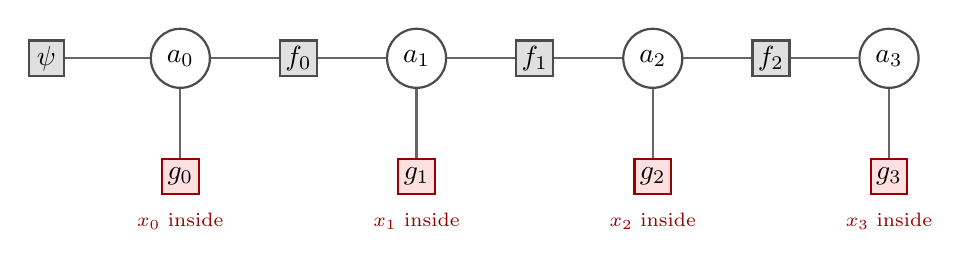
\begin{tikzpicture}[node distance=12mm]
  \node[fac] (pr) at (-1.7,0) {$\psi$};
  \node[var] (a0) at (0,0) {$a_0$};
  \node[fac] (f0) at (1.5,0) {$f_0$};
  \node[var] (a1) at (3,0) {$a_1$};
  \node[fac] (f1) at (4.5,0) {$f_1$};
  \node[var] (a2) at (6,0) {$a_2$};
  \node[fac] (f2) at (7.5,0) {$f_2$};
  \node[var] (a3) at (9,0) {$a_3$};
  \node[obs] (g0) at (0,-1.5) {$g_0$};
  \node[obs] (g1) at (3,-1.5) {$g_1$};
  \node[obs] (g2) at (6,-1.5) {$g_2$};
  \node[obs] (g3) at (9,-1.5) {$g_3$};
  \draw[e] (pr)--(a0)--(f0)--(a1)--(f1)--(a2)--(f2)--(a3);
  \draw[e] (a0)--(g0); \draw[e] (a1)--(g1);
  \draw[e] (a2)--(g2); \draw[e] (a3)--(g3);
  \node[below=1mm of g0, font=\scriptsize, red!60!black] {$x_0$ inside};
  \node[below=1mm of g1, font=\scriptsize, red!60!black] {$x_1$ inside};
  \node[below=1mm of g2, font=\scriptsize, red!60!black] {$x_2$ inside};
  \node[below=1mm of g3, font=\scriptsize, red!60!black] {$x_3$ inside};
\end{tikzpicture}
\end{center}

\noindent The graph for $K=4$: a backbone of variables and transition
factors, one observation leaf hanging off each variable, the prior capping
the left end --- ``a straight line with things on the side,'' exactly the
geometry described in the call. Counting: $K$ variables and $2K$ factors
($1$ prior, $K{-}1$ transitions, $K$ observations) make $3K$ nodes; the
edges are $2(K{-}1)$ from transitions (each touches two variables), $K$ from
observations, $1$ from the prior: $3K-1$ edges in total. A connected graph
with one fewer edge than nodes is a \emph{tree} --- no cycles. This single
combinatorial fact is what will make BP exact: on a tree, information has
exactly one route between any two nodes, so nothing can ever be counted
twice.

% =============================================================================
\section{Belief propagation, equation by equation}\label{sec:bp}
% =============================================================================

\subsection{The general sum--product equations, and where they hurt}
\label{sec:sumproduct}

BP computes, for every variable, its marginal posterior --- here
$p(a_k\given x)$, whose mean feeds \eqref{eq:tweedie}. It does so by passing
\emph{messages} along the edges of the factor graph. There are two kinds.

A \textbf{variable-to-factor} message: variable $a_i$ tells factor
$\psi_c$ what it currently believes about itself, based on everyone
\emph{except} $\psi_c$:
\begin{equation}\label{eq:v2f}
  \nu_{i\to c}(a_i)\ \propto\
  \prod_{b\,\in\,\partial i\setminus c}\hat\nu_{b\to i}(a_i) .
  \tag{SP1}
\end{equation}
Here $\partial i$ is the set of factors touching $a_i$, and the product runs
over all of them \emph{except the recipient} $c$ --- the recipient must not
hear its own previous opinion echoed back, or information would circulate
and inflate.

A \textbf{factor-to-variable} message: factor $\psi_c$ tells variable
$a_i$ what the factor implies about it, after averaging over the factor's
\emph{other} arguments, each weighted by what that argument currently
believes:
\begin{equation}\label{eq:f2v}
  \hat\nu_{c\to i}(a_i)\ \propto\
  \int\psi_c(a_{\partial c})
  \prod_{j\,\in\,\partial c\setminus i}\nu_{j\to c}(a_j)\;
  \dd a_{\partial c\setminus i} .
  \tag{SP2}
\end{equation}

The \textbf{belief} (the marginal estimate) at variable $a_i$ multiplies
everything that arrives:
\begin{equation}\label{eq:belief}
  b_i(a_i)\ \propto\ \prod_{c\,\in\,\partial i}\hat\nu_{c\to i}(a_i) .
  \tag{SP3}
\end{equation}
On a tree, the beliefs are \emph{exactly} the true marginals once each edge
has carried one message in each direction.

Now the difficulty named in the call. Every message above is a probability
distribution in its argument, defined ``up to proportionality'' --- meaning
it must be normalised. If $a_i$ takes $q$ discrete values, a message is a
vector of $q$ numbers; \eqref{eq:v2f} is an entrywise product,
\eqref{eq:f2v} a finite sum, normalisation a division by the total. If
$a_i$ is \emph{continuous}, a message is a \emph{function} on $\R$:
\eqref{eq:f2v} is an integral transform, and the normalising constant is
itself an integral that changes at every update. Propagating arbitrary
functions and renormalising them numerically, at every edge and every step,
is the intractability that motivated the call.

\subsection{The two facts that rescue the continuous case here}
\label{sec:lemmas}

For \emph{this} model every factor in \eqref{eq:factors} is Gaussian, and
two elementary facts about Gaussians close the algebra. We state and prove
both; together they will guarantee that every message in
\eqref{eq:v2f}--\eqref{eq:belief} is an (unnormalised) Gaussian, hence
carried by two numbers --- and the normalisation problem evaporates, because
a Gaussian normalises itself: its constant is determined by its (mean,
variance) pair and never needs to be tracked.

\begin{lemma}[products]\label{lem:prod}
For any means $m_1,m_2$ and variances $v_1,v_2$,
\[
  \N(a;m_1,v_1)\cdot\N(a;m_2,v_2)\ \propto\ \N(a;m,v),
  \qquad
  \frac1v=\frac1{v_1}+\frac1{v_2},
  \qquad
  \frac mv=\frac{m_1}{v_1}+\frac{m_2}{v_2} .
\]
\end{lemma}
\begin{proof}
Write each factor as $\exp(-\frac{a^2}{2v_i}+\frac{m_i}{v_i}a+\text{const})$.
The product adds the exponents, so the coefficient of $-a^2/2$ is
$1/v_1+1/v_2$ and the coefficient of $a$ is $m_1/v_1+m_2/v_2$. Any function
of the form $\exp(-\lambda a^2/2+\theta a)$ is proportional to
$\N(a;\theta/\lambda,1/\lambda)$.
\end{proof}

\noindent In words: \emph{precisions add; precision-weighted means add.}
This is the engine of every ``combine'' step below.

\begin{lemma}[linear propagation]\label{lem:lin}
For any $\alpha\neq0$, $s^2>0$:
\[
  \text{(forward)}\quad
  \int\N(a';\alpha a,s^2)\,\N(a;m,v)\,\dd a=\N(a';\alpha m,\ \alpha^2v+s^2),
\]
\[
  \text{(backward)}\quad
  \int\N(a';\alpha a,s^2)\,\N(a';m,v)\,\dd a'\ \propto\
  \N\!\Big(a;\ \frac m\alpha,\ \frac{v+s^2}{\alpha^2}\Big).
\]
\end{lemma}
\begin{proof}
Forward: the integral is the density of $a'=\alpha a+\eta$ where
$a\sim\N(m,v)$ and $\eta\sim\N(0,s^2)$ are independent; a linear
combination of independent Gaussians is Gaussian with mean $\alpha m$ and
variance $\alpha^2v+s^2$. Backward: viewed as a function of $a$, the first
factor satisfies $\N(a';\alpha a,s^2)\propto\N(a;a'/\alpha,s^2/\alpha^2)$
(divide the exponent's argument by $\alpha$), so the integral is the forward
case run through the inverted map $a=(a'-\eta)/\alpha$, giving mean
$m/\alpha$ and variance $(v+s^2)/\alpha^2$.
\end{proof}

\subsection{Specialising the equations to the chain}\label{sec:special}

We now instantiate \eqref{eq:v2f}--\eqref{eq:belief} on the factor graph of
Step~4.3, edge by edge, and watch most of them collapse.

\paragraph{Step 5.1: messages from leaf factors are just the factors.}
The prior $\psi$ and each observation $g_k$ touch a single variable, so in
\eqref{eq:f2v} there is nothing to integrate and no incoming message to
weight: $\hat\nu_{\psi\to a_0}(a_0)=\psi(a_0)=\N(a_0;0,1)$ and
$\hat\nu_{g_k\to a_k}(a_k)=g_k(a_k)$, the pseudo-observation
\eqref{eq:evidence}. Leaves simply inject their factor.

\paragraph{Step 5.2: messages along the backbone, and the bookkeeping.}
Consider the edge from variable $a_k$ into the transition factor $f_k$ (to
its right). Rule \eqref{eq:v2f} says: multiply everything arriving at $a_k$
except from $f_k$ --- that is, the message from the left transition
$f_{k-1}$ (or the prior, if $k=0$) and the message from the observation
$g_k$:
\begin{equation}\label{eq:nu-bk}
  \nu_{a_k\to f_k}(a_k)\ \propto\
  \hat\nu_{f_{k-1}\to a_k}(a_k)\cdot g_k(a_k) .
\end{equation}
Then rule \eqref{eq:f2v} at $f_k$, whose other argument is $a_{k+1}$:
\begin{equation}\label{eq:nuhat-bk}
  \hat\nu_{f_k\to a_{k+1}}(a_{k+1})
  =\int f_k(a_k,a_{k+1})\,\nu_{a_k\to f_k}(a_k)\,\dd a_k .
\end{equation}
Define the \emph{forward message}
$\mu_{\to k}:=\hat\nu_{f_{k-1}\to a_k}$ (with
$\mu_{\to0}:=\hat\nu_{\psi\to a_0}$) and substitute \eqref{eq:nu-bk} into
\eqref{eq:nuhat-bk}. The two-rule dance collapses into a single recursion,
which we now write with every operation labelled:
\begin{align}
  &\mu_{\to0}(a_0)=\N(a_0;0,1)
  &&\text{(start: the prior)}
  \tag{F0}\label{eq:F0}\\[2pt]
  &\text{combine: }(m^c_k,v^c_k)
  =\text{Lemma \ref{lem:prod}}\big[\mu_{\to k}\,,\;g_k\big]
  &&\text{(absorb the local data $x_k$)}
  \tag{F1}\label{eq:F1}\\[2pt]
  &\mu_{\to k+1}(a_{k+1})
  =\N\!\big(a_{k+1};\ \alpha m^c_k,\ \alpha^2v^c_k+\sigma_\eta^2\big)
  &&\text{(Lem.~\ref{lem:lin}, fwd)}
  \tag{F2}\label{eq:F2}
\end{align}
Spelled out, \eqref{eq:F1} reads: with the pseudo-observation
\eqref{eq:evidence},
\[
  \frac1{v^c_k}=\frac1{v_{\to k}}+\frac{e^{-2t}}{D_t},
  \qquad
  \frac{m^c_k}{v^c_k}=\frac{m_{\to k}}{v_{\to k}}+\frac{e^{-t}}{D_t}x_k .
\]
By symmetry, peeling the chain from the right gives the \emph{backward
message} $\mu_{\leftarrow k}:=\hat\nu_{f_k\to a_k}$:
\begin{align}
  &\mu_{\leftarrow K-1}(a_{K-1})\equiv1
  &&\text{(start: nothing right of the end --- flat)}
  \tag{B0}\label{eq:B0}\\[2pt]
  &\text{combine: }(m^c_k,v^c_k)
  =\text{Lemma \ref{lem:prod}}\big[\mu_{\leftarrow k}\,,\;g_k\big]
  &&\text{(absorb $x_k$)}
  \tag{B1}\label{eq:B1}\\[2pt]
  &\mu_{\leftarrow k-1}(a_{k-1})
  =\N\!\Big(a_{k-1};\ \tfrac{m^c_k}{\alpha},\
  \tfrac{v^c_k+\sigma_\eta^2}{\alpha^2}\Big)
  &&\text{(Lem.~\ref{lem:lin}, bwd)}
  \tag{B2}\label{eq:B2}
\end{align}
The flat start \eqref{eq:B0} is the $v\to\infty$ limit of a Gaussian
(precision $0$); Lemma \ref{lem:prod} handles it exactly --- multiplying by
a flat message changes nothing.

Finally the belief \eqref{eq:belief} at node $k$ multiplies the three
arrivals --- left transition, observation, right transition:
\begin{equation}\label{eq:C}
  p(a_k\given x)\ \propto\
  \mu_{\to k}(a_k)\;\cdot\;g_k(a_k)\;\cdot\;\mu_{\leftarrow k}(a_k),
  \tag{C}
\end{equation}
two applications of Lemma \ref{lem:prod}. Its mean is $\E[a_k\given x]$,
which enters Tweedie \eqref{eq:tweedie} to give the score.

\begin{remark}[the one trap, stated loudly]\label{rmk:trap}
In \eqref{eq:F1} the local observation $g_k$ is absorbed \emph{when
leaving} node $k$, so the forward message $\mu_{\to k}$ \emph{arriving} at
node $k$ contains the data $x_0,\dots,x_{k-1}$ and \textbf{not} $x_k$;
symmetrically $\mu_{\leftarrow k}$ contains $x_{k+1},\dots,x_{K-1}$ and not
$x_k$. The combination \eqref{eq:C} then counts $x_k$ exactly once --- via
its own factor $g_k$. The tempting shortcut of folding $g_k$ \emph{into}
the stored message $\mu_{\to k}$ makes \eqref{eq:C} count $x_k$ twice and
silently corrupts every marginal. This bookkeeping is forced by the
$\setminus c$ exclusions in \eqref{eq:v2f}--\eqref{eq:f2v}; it is the
single most error-prone point of an implementation, which is why the code
states it in its header comment and the checks of \S\ref{sec:checkpoint}
would catch the violation at order one.
\end{remark}

\paragraph{Step 5.3: the algorithm, assembled.}
\begin{center}
\fbox{\parbox{0.92\textwidth}{\small
\textbf{Gaussian BP on the AR(1) diffusion chain.} Input: $x\in\R^K$,
$\alpha$, $t$.\\[2pt]
1.\ \textbf{Forward sweep} (left to right): start with \eqref{eq:F0};
for $k=0,\dots,K{-}2$ apply \eqref{eq:F1} then \eqref{eq:F2}. Store
$(m_{\to k},v_{\to k})$ for every $k$.\\
2.\ \textbf{Backward sweep} (right to left): start with \eqref{eq:B0};
for $k=K{-}1,\dots,1$ apply \eqref{eq:B1} then \eqref{eq:B2}. Store
$(m_{\leftarrow k},v_{\leftarrow k})$.\\
3.\ \textbf{Combine} at every $k$ with \eqref{eq:C}: posterior mean $m_k$
and variance $v_k$.\\
4.\ \textbf{Score} by Tweedie \eqref{eq:tweedie}:
$S_k=(e^{-t}m_k-x_k)/D_t$.\\[2pt]
Cost: each sweep is $K{-}1$ constant-cost updates on number pairs; total
$O(K)$, against the $O(K^3)$ of solving \eqref{eq:score-exact} naively.}}
\end{center}

\subsection{Are the messages Gaussian? Are we approximating?}
\label{sec:gaussianity}

\begin{claim}\label{claim:closure}
On this model, every message and every belief produced by
\eqref{eq:F0}--\eqref{eq:C} is exactly Gaussian (or flat), at every node and
every $(K,\alpha,t)$. The two-number parametrisation is therefore lossless:
\emph{Gaussian BP here is BP}, with no approximation anywhere.
\end{claim}
\begin{proof}
Induction along each sweep. Base cases: \eqref{eq:F0} is Gaussian;
\eqref{eq:B0} is the flat limit. Induction step: \eqref{eq:F1}/\eqref{eq:B1}
are products of two Gaussians (Lemma \ref{lem:prod}: Gaussian);
\eqref{eq:F2}/\eqref{eq:B2} are linear-Gaussian integrals (Lemma
\ref{lem:lin}: Gaussian). The combination \eqref{eq:C} is a double product
(Gaussian). No step ever leaves the family.
\end{proof}

This settles the call's first question \emph{for this model}, and the
mechanism is worth stating because it transfers: the closure holds because
every operation the graph demands --- multiply two Gaussians in the same
variable, push a Gaussian through a \emph{linear} transition with Gaussian
noise --- is an operation under which the Gaussian family is invariant. It
is an \emph{algebraic} property of the factors, valid at any node degree,
including degree two. No central limit theorem was invoked, so there is no
``CLT on two points'' to fail. (The criterion proposed in the call is
exactly right: the updates here are linear in the propagated statistics ---
had the transition been nonlinear, $a_{k+1}=\phi(a_k)+\eta_k$, Lemma
\ref{lem:lin} would fail and the messages would leave the Gaussian family;
\emph{that} is the case where Gaussian parametrisation becomes a genuine
approximation.)

\begin{question}
If the message at each node is Gaussian, is the joint distribution of the
whole sequence Gaussian? (Raised in the call: ``it's not entirely trivial
\dots\ you've updated everyone with everyone else.'')
\end{question}
\begin{answer}
The implication is false in general, and the doubt is correct: marginal
Gaussianity does not imply joint Gaussianity (a standard counterexample
couples two standard Gaussians through a non-Gaussian copula --- both
marginals are exactly $\N(0,1)$, the pair is not jointly Gaussian). BP
messages and beliefs are \emph{per-node marginal} objects; nothing about
their shape constrains the joint law. For \emph{our} posterior the joint
\emph{is} Gaussian, but for a reason independent of message passing: the
log-density \eqref{eq:posterior} is a quadratic form in $a$, globally. The
correct logic is therefore: joint Gaussianity comes from the model
(quadratic log-density); message Gaussianity then follows from it (any
marginal or conditional of a joint Gaussian is Gaussian); never the reverse.
\end{answer}

\subsection{The checkpoint: BP recovers the exact score}
\label{sec:checkpoint}

The call's proposed test: run the message passing on the solvable case and
compare with the known answer. We run it on a worked instance small enough
to print every number, then sweep the parameter space.

\paragraph{A complete instance.} $K=4$, $\alpha=0.6$, $t=0.3$,
$x=(0.9,\,-0.2,\,0.5,\,-1.1)$, so $e^{-t}=0.740818$, $D_t=0.451188$,
$\sigma_\eta^2=0.64$, pseudo-observation variance $D_te^{2t}=0.822119$.
Running \eqref{eq:F0}--\eqref{eq:C}:

\begin{center}\footnotesize
\setlength{\tabcolsep}{4pt}
\begin{tabular}{@{}lcccc@{}}
\toprule
 & $k=0$ & $k=1$ & $k=2$ & $k=3$\\
\midrule
forward $\mu_{\to k}$ (m, v) & $(0,\,1)$ & $(0.40004,\,0.80243)$
  & $(0.04146,\,0.78619)$ & $(0.21067,\,0.78468)$\\
pseudo-obs.\ \eqref{eq:evidence} (m, v) & $(1.21487,\,0.82212)$
  & $(-0.26997,\,0.82212)$ & $(0.67493,\,0.82212)$
  & $(-1.48485,\,0.82212)$\\
backward $\mu_{\leftarrow k}$ (m, v) & $(-0.29429,\,3.64415)$
  & $(0.24117,\,3.67700)$ & $(-2.47474,\,4.06144)$ & flat\\
\midrule
posterior (mean, var) & $(0.56086,\,0.40148)$ & $(0.08621,\,0.36569)$
  & $(0.09668,\,0.36569)$ & $(-0.61733,\,0.40148)$\\
\bottomrule
\end{tabular}
\end{center}

\noindent
One step verified by hand so the table is auditable. Forward into $k=1$:
combine \eqref{eq:F0} with the pseudo-observation at $k=0$ (Lemma
\ref{lem:prod}): precision $1+1/0.82212=2.21637$, variance $0.45119$,
mean $0.45119\times(0+1.21487/0.82212)=0.66673$; then \eqref{eq:F2}:
mean $0.6\times0.66673=0.40004$, variance
$0.36\times0.45119+0.64=0.80243$. Matches the table. The
Tweedie line \eqref{eq:tweedie} then gives
\[
  S^{\textsc{bp}}(x,t)=(-1.07384,\ 0.58482,\ -0.94945,\ 1.42439),
\]
and the matrix benchmark \eqref{eq:score-exact} gives the same four numbers
to all printed digits. Note also the symmetry $v_0=v_3$ and $v_1=v_2$ in
the posterior variances --- variances do not depend on the data $x$, only
on the geometry, and the chain is symmetric under reversal.

\paragraph{The sweep.} Over $K\in\{2,3,6,12\}$,
$\alpha\in\{0.3,0.7,0.9,-0.5\}$, $t\in\{0.05,0.4,1.2,3\}$ with random $x$
(64 configurations), the largest deviation between the BP pipeline and the
exact computation is
\begin{align*}
  \max\big|m^{\textsc{bp}}_k-(J^{-1}h)_k\big|&=2.0\times10^{-15},&
  \max\big|v^{\textsc{bp}}_k-(J^{-1})_{kk}\big|&=2.4\times10^{-15},\\
  \max\big|S^{\textsc{bp}}_k-S_k\big|&=9.8\times10^{-15}.&&
\end{align*}
This is double-precision rounding. \textbf{The checkpoint passes}: the
message-passing algorithm with two-number Gaussian messages reproduces the
solved case exactly, as conjectured in the call --- and
Claim~\ref{claim:closure} explains why the agreement is exact rather than
approximate.

% =============================================================================
\section{AMP: the per-node Gaussian field, and what it costs}\label{sec:amp}
% =============================================================================

\subsection{From per-edge messages to per-node statistics}

The call's description of the general recipe: when the BP updates are
intractable, parametrise the local distributions as Gaussians and ``reduce
everything to a mean and variance update.'' The fully reduced scheme --- AMP
/ TAP --- goes one step further than \S\ref{sec:special}: instead of a
(mean, variance) pair \emph{per directed edge} (our $\mu_{\to k}$,
$\mu_{\leftarrow k}$), it keeps a single pair $(m_i,V_i)$ \emph{per node}
and updates it against the aggregate of all neighbours. Working on the
posterior in natural parameters \eqref{eq:posterior} --- precision $J$
(tridiagonal), field $h$ --- the per-node updates read
\begin{align}
  m_i\ &\leftarrow\
  \frac{1}{J_{ii}}\Big(h_i-\sum_{j\neq i}J_{ij}\,m_j\Big),
  \tag{A1}\label{eq:A1}\\[2pt]
  V_i\ &\leftarrow\
  \frac{1}{\,J_{ii}-\sum_{j\neq i}J_{ij}^2\,V_j\,}.
  \tag{A2}\label{eq:A2}
\end{align}
Where these come from, stated without mystery: node $i$ models the combined
effect of its neighbours as a Gaussian field. For the \emph{mean}, the
stationarity condition of \eqref{eq:A1} is literally the $i$-th row of
$Jm=h$. For the \emph{variance}, each neighbour $j$ contributes its current
uncertainty $V_j$ propagated through the coupling $J_{ij}$ (squared,
because variances add under linear maps), and \eqref{eq:A2} is the
self-consistent solution --- with the crucial simplification that node $i$
uses the neighbour's \emph{full} variance $V_j$, not the variance the
neighbour would have \emph{if $i$ were absent} (the per-edge, ``cavity''
quantity that true BP keeps). Dropping that exclusion is exactly what makes
the scheme per-node instead of per-edge; it is harmless when each node has
many weak neighbours --- removing one of $N$ changes little, and the
aggregated field is near-Gaussian by the central limit theorem, with the
$1/\sqrt N$ convergence noted in the call --- and it is an order-one
modification when the neighbours number two.

\subsection{What survives: the score}

\begin{claim}\label{claim:samescore}
Any fixed point of \eqref{eq:A1} satisfies $Jm=h$ exactly --- the same
linear system whose solution is the true posterior mean. The variance
update \eqref{eq:A2} does not enter \eqref{eq:A1} at all. Hence AMP's mean,
wherever its iteration converges, equals the exact posterior mean, and by
Tweedie \eqref{eq:tweedie} \textbf{AMP's score equals the exact score}, at
every diffusion time --- regardless of how wrong, or even nonexistent, its
variances are.
\end{claim}

Measured (chain, $K=12$, $\alpha=0.8$; damped iteration of
\eqref{eq:A1}): the gap between the AMP mean and the exact mean is below
$3\times10^{-12}$ at every tested $t$. For the \emph{score} --- the object
diffusion needs --- the Gaussian local-field approximation on this model is
not an approximation at all.

\subsection{What breaks: the variance}\label{sec:amp-variance}

The variance closure \eqref{eq:A2} is genuinely different from BP's, and on
a two-neighbour chain the difference is visible in one line. In the
homogeneous interior of a long chain, $J$ has constant diagonal
$J_{\mathrm d}=e^{-2t}/D_t+(1+\alpha^2)/\sigma_\eta^2$ and constant
off-diagonal $\beta=-\alpha/\sigma_\eta^2$. BP's per-edge variance
bookkeeping --- one neighbour excluded --- has fixed points solving
\[
  \lambda=J_{\mathrm d}-\frac{\beta^2}{\lambda}
  \quad\Longleftrightarrow\quad
  \lambda^2-J_{\mathrm d}\lambda+\beta^2=0,
\]
with real solutions iff $J_{\mathrm d}^2\ge4\beta^2$ --- which always holds,
since $J_{\mathrm d}-2|\beta|
=e^{-2t}/D_t+(1-|\alpha|)^2/\sigma_\eta^2>0$. The per-node closure
\eqref{eq:A2} --- both neighbours included --- has fixed points solving
\[
  V=\frac1{J_{\mathrm d}-2\beta^2V}
  \quad\Longleftrightarrow\quad
  2\beta^2V^2-J_{\mathrm d}V+1=0,
\]
with real solutions iff $J_{\mathrm d}^2\ge8\beta^2$. The entire difference
between BP and AMP on this chain is the factor $2$ --- the dropped
exclusion --- and it moves the existence threshold from ``always'' to a
condition that \emph{fails} once the prior coupling dominates the evidence,
i.e.\ at large enough $t$ for strong enough $\alpha$. Beyond that point the
bracket in \eqref{eq:A2} turns negative during the iteration: there is no
positive fixed point, and the honest report is failure, not a clipped
number. Measured breakdown times of the iteration ($K=200$, bisection):
\begin{gather*}
  \alpha=0.5:\ t\approx0.86,\qquad
  \alpha=0.7:\ t\approx0.36,\qquad
  \alpha=0.9:\ t\approx0.11,\\
  \alpha=0.3:\ \text{no breakdown found up to }t=30 .
\end{gather*}
This is the precise content of the call's objection: the central limit
argument that justifies treating the aggregated neighbour field as an
independent Gaussian is a many-neighbour argument, and on two neighbours
its failure is not a small distortion --- beyond a threshold the
self-consistent variance simply ceases to exist. But note exactly
\emph{where} the objection lands: on the variance \eqref{eq:A2}, never on
the mean \eqref{eq:A1}, whose fixed-point equation is closure-independent.
The ``CLT on two points'' worry is correct, and the score survives it.

% =============================================================================
\section{Experiment 1: how bad is locality?}\label{sec:exp1}
% =============================================================================

The exact score matrix $Q_t=\Sigma_t^{-1}$ is full for every $t>0$:
inference at one frame draws on all frames. The call proposed to quantify
the cost of pretending otherwise, in two distinct ways that we keep
carefully apart.

\paragraph{Variant 1a --- truncate the matrix.} Replace $Q_t$ by
$Q_t^{(b)}$, keeping only entries with $|i-j|\le b$ ($b=1$ is the
tridiagonal truncation suggested in the call), and use
$\hat S(x)=-Q_t^{(b)}x$.

\paragraph{Variant 1b --- truncate the inference.} ``Cut the iteration'':
let messages travel at most $r$ hops, replacing any message from beyond the
cut by its no-evidence value --- the stationary prior. Concretely, the
estimate of $a_k$ uses exact inference on the window
$x_{k-r},\dots,x_{k+r}$ alone (a contiguous block of the stationary chain
is itself a stationary AR(1) chain, so the windowed problem is again of the
same form); the score follows by Tweedie.

\paragraph{The error measure, with no randomness.} Every estimator above is
\emph{linear} in $x$: $\hat S(x)=-Mx$ for a computable matrix $M$, while
the truth is $S(x)=-Q_tx$. Averaging over the data distribution
$x\sim P_t=\N(0,\Sigma_t)$, the mean squared error is a trace
(using $\E[x\T Ax]=\tr(A\Sigma_t)$ for any matrix $A$):
\[
  \E\big\|\hat S(x)-S(x)\big\|^2
  =\tr\!\big((M-Q_t)\,\Sigma_t\,(M-Q_t)\T\big),
  \qquad
  \E\|S(x)\|^2=\tr\!\big(Q_t\Sigma_tQ_t\big)=\tr Q_t ,
\]
and we report the \emph{relative root error} --- the square root of the
ratio. No samples, no seeds: each point in the figures is a deterministic
number.

\begin{figure}[t]\centering
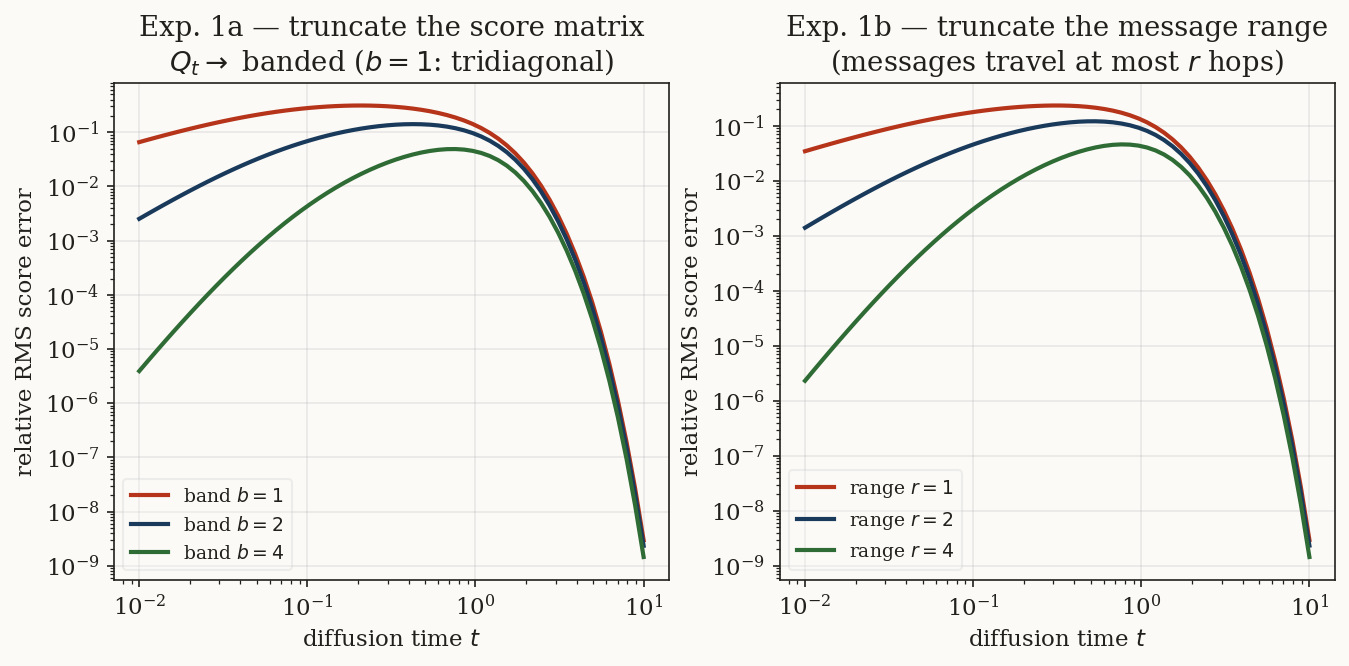
\includegraphics[width=\linewidth]{figures/exp1_truncation.png}
\caption{Relative RMS score error of the two truncations
($K=40$, $\alpha=0.8$) as a function of diffusion time. Left: banded score
matrix, $b\in\{1,2,4\}$. Right: truncated message range,
$r\in\{1,2,4\}$.}
\label{fig:exp1}
\end{figure}

\begin{figure}[t]\centering
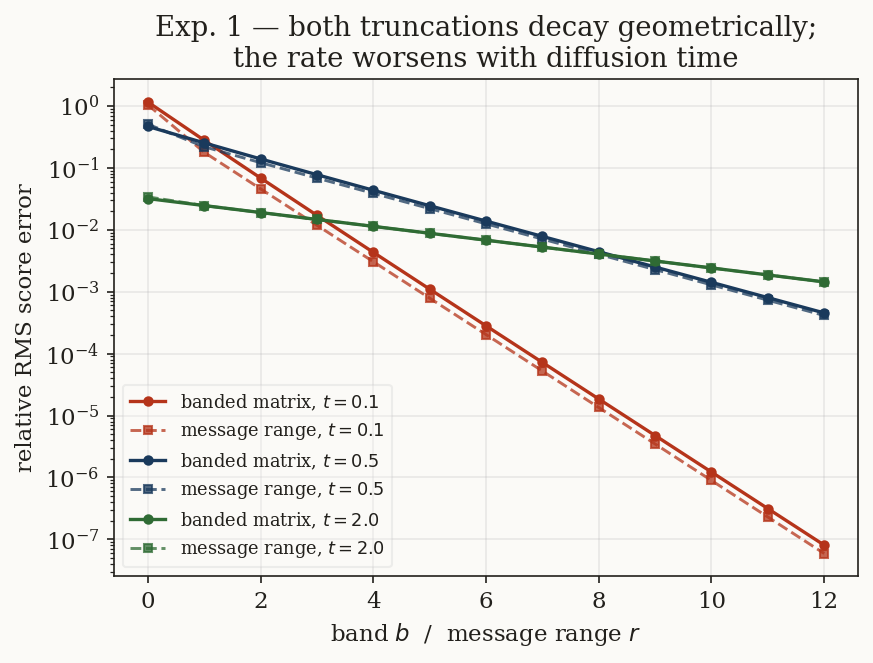
\includegraphics[width=0.62\linewidth]{figures/exp1_vs_radius.png}
\caption{The same errors as a function of the band / range at three fixed
times. Both truncations converge geometrically as the allowed range grows;
the rate is fast at $t=0.1$, slowest near $t\sim0.5$.}
\label{fig:exp1b}
\end{figure}

\paragraph{Findings.} (Figures \ref{fig:exp1}--\ref{fig:exp1b}; selected
values for $b=r=1$, $K=40$, $\alpha=0.8$.)
\begin{center}\small
\begin{tabular}{@{}lcccc@{}}
\toprule
relative RMS error & $t=0.05$ & $t=0.3$ & $t=1$ & $t=3$\\
\midrule
1a: tridiagonal matrix ($b=1$) & $0.210$ & $0.302$ & $0.135$ & $0.0035$\\
1b: message range $r=1$        & $0.123$ & $0.235$ & $0.130$ & $0.0035$\\
\bottomrule
\end{tabular}
\end{center}

\begin{enumerate}[leftmargin=1.7em, itemsep=2pt]
\item \textbf{The cost of locality is non-monotone in $t$ and peaks at
intermediate times.} At $t\to0$ the score is genuinely near-tridiagonal
(the posterior precision is $Q_0$ plus a large diagonal), and at
$t\to\infty$ the score decouples entirely ($Q_t\to I$, $S\to-x$); in
between, the truncated estimator misses up to $\sim30\%$ of the score in
RMS. This confirms quantitatively the intuition discussed in the call: the
matrix ``starts tridiagonal, becomes full at intermediate times'' --- and
intermediate times are where locality genuinely hurts.
\item \textbf{Truncated inference beats the truncated matrix at small $t$,
at equal locality.} At $t=0.05$: $12.3\%$ versus $21.0\%$. The reason is
worth recording: variant 1b solves a \emph{correctly normalised} inference
problem on the window (the window's own prior block), while variant 1a
zeroes entries of an inverse, which is not the inverse of anything and in
particular misstates the diagonal. Cutting the \emph{algorithm} is better
than cutting the \emph{answer}. The two coincide at large $t$, where all
off-diagonal content dies anyway.
\item \textbf{The error decays geometrically in the allowed range}
(Fig.~\ref{fig:exp1b}), with a rate that worsens as $t$ grows toward the
intermediate regime: each extra hop of message range buys a fixed
multiplicative factor of accuracy, and the factor is closest to $1$
precisely where the band of $Q_t$ is fullest.
\item \textbf{Architecture reading} (the call's motivation): a score
network with a restrained, local receptive field --- patches, a CNN --- is
near-optimal at small and large diffusion times, and pays a quantifiable
price (here up to $\sim30\%$ RMS at range $1$, $\sim13\%$ at range $2$,
$\sim5\%$ at range $4$) in the mid-diffusion window. If the architecture's
range can grow with $t$ --- or simply be sized for the worst time --- the
locality of the underlying Markov data is exploitable essentially for
free.
\end{enumerate}

% =============================================================================
\section{Experiment 2: AMP against the exact score}\label{sec:exp2}
% =============================================================================

The second comparison asked in the call: the Gaussian local-field
approximation against the truth, on the chain. We iterate \eqref{eq:A1}
and \eqref{eq:A2} (damping $0.5$) and compare with the exact posterior
mean and variances; Fig.~\ref{fig:exp2} and the table give the result
($K=12$, $\alpha=0.8$).

\begin{figure}[t]\centering
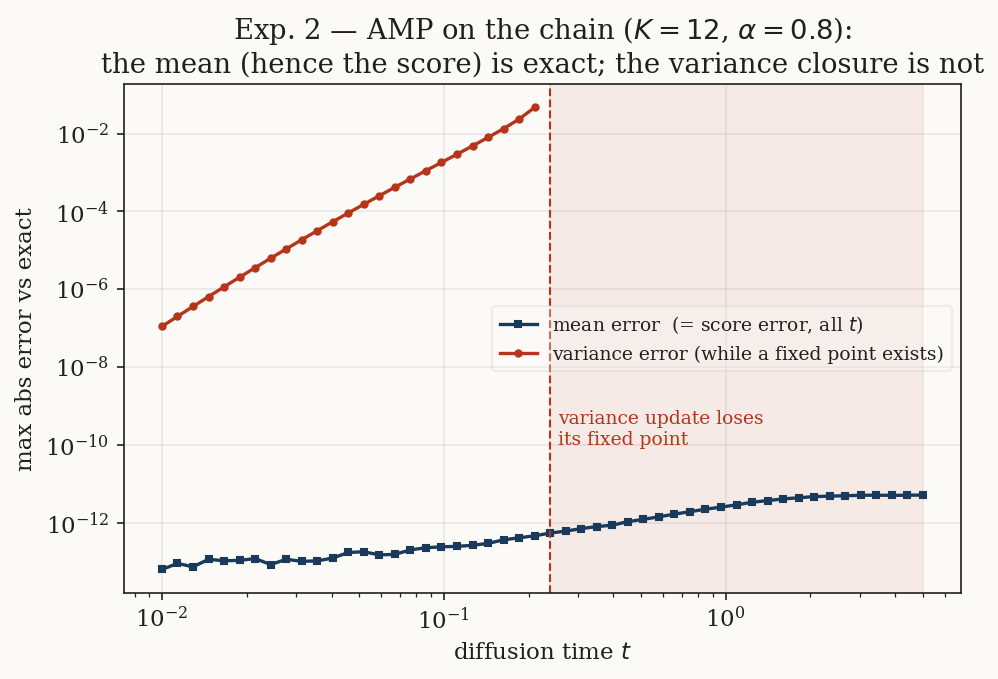
\includegraphics[width=0.72\linewidth]{figures/exp2_amp.png}
\caption{AMP on the chain. The mean error (navy) sits at numerical noise
for every diffusion time --- the score is exact, Claim
\ref{claim:samescore}. The variance error (red) grows steadily with $t$
and, past $t\approx0.23$, the update \eqref{eq:A2} has no positive fixed
point at all (shaded).}
\label{fig:exp2}
\end{figure}

\begin{center}\small
\begin{tabular}{@{}lcc@{}}
\toprule
$t$ & mean (= score) error & variance error\\
\midrule
$0.05$ & $1.8\times10^{-13}$ & $1.3\times10^{-4}$\\
$0.2$  & $4.7\times10^{-13}$ & $3.5\times10^{-2}$\\
$0.5$  & $1.2\times10^{-12}$ & no fixed point\\
$1.0$  & $2.6\times10^{-12}$ & no fixed point\\
\bottomrule
\end{tabular}
\end{center}

\paragraph{Verdict.} The two halves of the call's intuition are both
confirmed, and they separate cleanly:
\begin{itemize}[leftmargin=1.7em, itemsep=2pt]
\item the conjecture --- run the Gaussian message passing on the solved
case and ``recover what we had'' --- holds \emph{exactly} for the score,
both for true BP (\S\ref{sec:checkpoint}, where it holds by algebraic
closure) and for AMP (Claim \ref{claim:samescore}, where it holds because
the mean update's fixed point is closure-independent);
\item the objection --- ``a CLT on two data points is usually not right''
--- is also exactly right, and its target is the \emph{variance} closure
\eqref{eq:A2}: accurate while the per-frame evidence dominates (small
$t$), degrading as the prior coupling takes over, and ceasing to exist
past a threshold time that shrinks as the chain coupling $\alpha$ grows
(\S\ref{sec:amp-variance}).
\end{itemize}
On this model one can therefore use the cheap per-node scheme for the
score with impunity, but must not trust --- past small $t$, must not even
expect to compute --- its uncertainties. Any application needing
calibrated posterior variances (likelihoods, error bars, exploration)
needs the per-edge messages of \S\ref{sec:special}, which cost the same
$O(K)$ and are exact.

% =============================================================================
\section{Summary, and what to bring to the next call}\label{sec:summary}
% =============================================================================

\paragraph{Established here.}
\begin{enumerate}[leftmargin=1.7em, itemsep=2pt]
\item The continuous-message obstruction dissolves for this model: every
sum--product message is exactly Gaussian (Claim \ref{claim:closure}),
because every update is one of two operations under which the Gaussian
family is closed. Two numbers per message; normalisation never tracked.
\item The checkpoint passes: Gaussian BP returns the known score to
$10^{-14}$, in $O(K)$, with every message derived
(\eqref{eq:F0}--\eqref{eq:C}) and printed on a worked instance.
\item Node-wise Gaussianity does not imply joint Gaussianity in general;
here the joint posterior is Gaussian because its log-density is quadratic
--- the implication runs from the model to the messages, not conversely.
\item AMP (per-node mean/variance) returns the \emph{same score} at every
$t$ --- the mean fixed point is $Jm=h$ regardless of the variance closure
--- while its variance is accurate only at small $t$ and has no fixed
point beyond a measurable threshold: the ``CLT on two points'' objection,
located precisely.
\item Locality costs at most $\sim30\%$ relative RMS (tridiagonal, worst
$t$) and almost nothing at small or large $t$; truncating the
\emph{inference} is uniformly no worse, and at small $t$ clearly better,
than truncating the \emph{matrix}.
\end{enumerate}

\paragraph{Next steps suggested by the call, in order of leverage.}
\begin{enumerate}[leftmargin=1.7em, itemsep=2pt]
\item \textbf{The discrete-data route.} Keep the Markov chain on a finite
alphabet (a transition matrix, no continuous innovation), add the Gaussian
channel only at diffusion. Messages become finite vectors, BP is exact and
trivially implementable, and the Bayes-optimal denoiser is computable ---
a second fully solvable pole, with non-Gaussian data, against which the
Gaussian-approximation questions can be asked sharply.
\item \textbf{Non-Gaussian innovations (e.g.\ Laplace).} Lemma
\ref{lem:lin} fails; messages leave the Gaussian family; projecting them
back (moment matching) makes Gaussian BP a genuine approximation. The
call's expectation --- the quality ``will strongly depend on the data
distribution'' --- becomes testable on the same factor graph, with the
same two experiments.
\item \textbf{Time-adaptive locality.} Experiment 1 gives, for each $t$,
the smallest range achieving a target error: a principled receptive-field
schedule for a restrained score architecture (the call's CNN/patches
remark), to be compared against what trained local networks actually
learn.
\end{enumerate}

\paragraph{Reproducibility.} Everything in this note is generated by two
files in this folder: \texttt{bp\_gaussian.py} (model, exact score, BP,
truncations, AMP, error metrics --- with built-in checks; run it) and
\texttt{experiments.py} (the figures and every number quoted). The
executed notebook \texttt{companion.ipynb} walks the same path
interactively. The bibliography is deliberately short: the two references
named in the call.

\begin{thebibliography}{9}
\bibitem{MM2009} M.~M\'ezard and A.~Montanari,
\emph{Information, Physics, and Computation}, Oxford University Press,
2009. Chapter 14 (belief propagation; the sum--product equations
14.14--14.15 discussed in the call).
\bibitem{ZK2021} L.~Zdeborov\'a and F.~Krzakala,
\emph{Statistical Physics for Optimization and Learning}, EPFL doctoral
lecture notes, 2021. (The Gaussian-parametrised message passing --- mean
and variance updates --- and the $1/\sqrt N$ central-limit control of the
aggregated field discussed in the call.)
\end{thebibliography}

\end{document}
